\chapter{Softwareumsetzung}
\label{cha:Software}

Mit Hilfe des in Kapitel \ref{sec:Kamera} beschriebenen Kameramoduls müssen verschiedene Aufgaben aus dem Bereich der Bildverarbeitung bewältigt werden. 

\section{Wahl der Bildverarbeitungsbibliothek}

Die Umsetzung der zu bewältigenden Aufgaben kann durch die Wahl einer geeigneten Bildverarbeitungsbibliothek deutlich vereinfacht werden. Wichtige Kriterien für die Wahl der Bibliothek sind unter anderem Funktionsumfang, Dokumentation und aktivität der Community.

\subsection{LibCCV}

LibCCV \cite{libccv} ist eine open-source Bildverarbeitungsbilbiothek, die viele bekannte Algorithmen implementiert. LibCCV steht unter einer BSD-Clause-3-Lizenz und kann somit für eine Studienarbeit problemlos unbegrenzt verwendet werden. Die Bibliothek ist größtenteils in C++ verfasst und somit potenziell auf einem Android-Smartphone verwendet werden. Die Verwendung auf dem Smartphone wird jedoch nicht offiziell unterstützt und kann potenziell weitere Schwierigkeiten mit sich bringen.

\subsection{Imagemagick}

Bei Imagemagick \cite{imagemagick} handelt es sich um eine Bildverarbeitungsbibliothek, welche sehr viele Algorithmen bereits implementiert hat. Algorithmen zur Objekterkennung müssten jedoch vollständig selbst implementiert werden, was zu einem großen zusätzlichen Aufwand führen kann. Imagemagick wird unter der Apache 2.0 Lizenz vertrieben.

\subsection{OpenCV}
\label{subsec:opencv}

OpenCV \cite{opencv_library, bradski2008learning} stellt eine der größten Open-Source-Bibliotheken für Bildverarbeitung da. Die Bibliothek hat einen starken Focus auf Echtzeitverarbeitung und wird daher auch in vielen Projekten im Bereich der Robotik verwendet. OpenCV hat eine große aktive Community, wodurch eventuelle Fragen und Probleme schnell beantwortet werden können. Zusätzlich bietet OpenCV eine offizielle Verison für Android und eignet sich somit ideal für diese Studienarbeit.


\section{Algorithmen zur Objekterkennung}
\label{sec:Objekterkennung}

Aufgabe des Roboters, ist es Gegenstände in einem Raum mit Hilfe von Kamerabildern zu erkennen. Folglich spielt die Objekterkennung eine große Rolle.

\subsection{Farbbasierte Objekterkennung}
Einen einfachen Ansatz der Objekterkennung unter Verwendung von Methoden der in \ref{subsec:opencv} beschriebenen Bibliothek OpenCV stellt eine farbbasierte Objekterkennung dar. Hierfür wird das Kamerabild zunächst vom RGB-Format [ZITAT EINFÜGEN] in das HSV-Format [ZITAT] konvertiert. Dies wird durchgeführt, da das HSV-Format unempfindlicher gegen Veränderungen in der Beleuchtung ist als das RGB-Format. Abbildung \ref{fig:ColorModels} zeigt die Aufteilung eines Bildes in die verschiedenen Kanäle.

\begin{figure}[h]
\centering
\includegraphics[width=\textwidth]{Bilder/Software/ColormodelsAll}
\caption{Beispiel einer Aufspaltung in RGB-Kanäle (links) und HSV-Kanäle (rechts)}
\label{fig:ColorModels}
\end{figure}

Wie in Abbildung \ref{fig:ColorModels} zu sehen ist, eignet sich vor allem der Saturation-Kanal des Bildes um farbige Objekte zu erkennen, da dieser hohe Werte annimmt wenn die Farbintensität hoch ist. Zuletzt erfolgt eine Binarisierung mit einem empirisch ermittelten Schwellwert von 50. Dies ist notwendig, da die, in der OpenCV-Bibliothek implementierte, Methode von Suzuki und Abe \cite{suzuki1985topological} zur Segmentierung von Objekten ein Binärbild erwartet. Aus dem in Abbildung \ref{fig:ColorModels} dargestellten Beispiel entsteht nach der Binarisierung schließlich Abbildung \ref{fig:BinarizedColorModels}. Der Algorithmus zur Segmentierung erkennt daraus drei Objekte und zeichnet ihren Konturen, wie in Abbildung \ref{fig:SegmentedColorModels} ersichtlich, ein.

\begin{figure}[h]
\centering

\includegraphics[width=\textwidth/2]{Bilder/Software/ColormodelsBinarized}
\caption{Beispiel der Binarisierung des Sättigungskanals}
\label{fig:BinarizedColorModels}
\end{figure}
\begin{figure}[h]
\centering
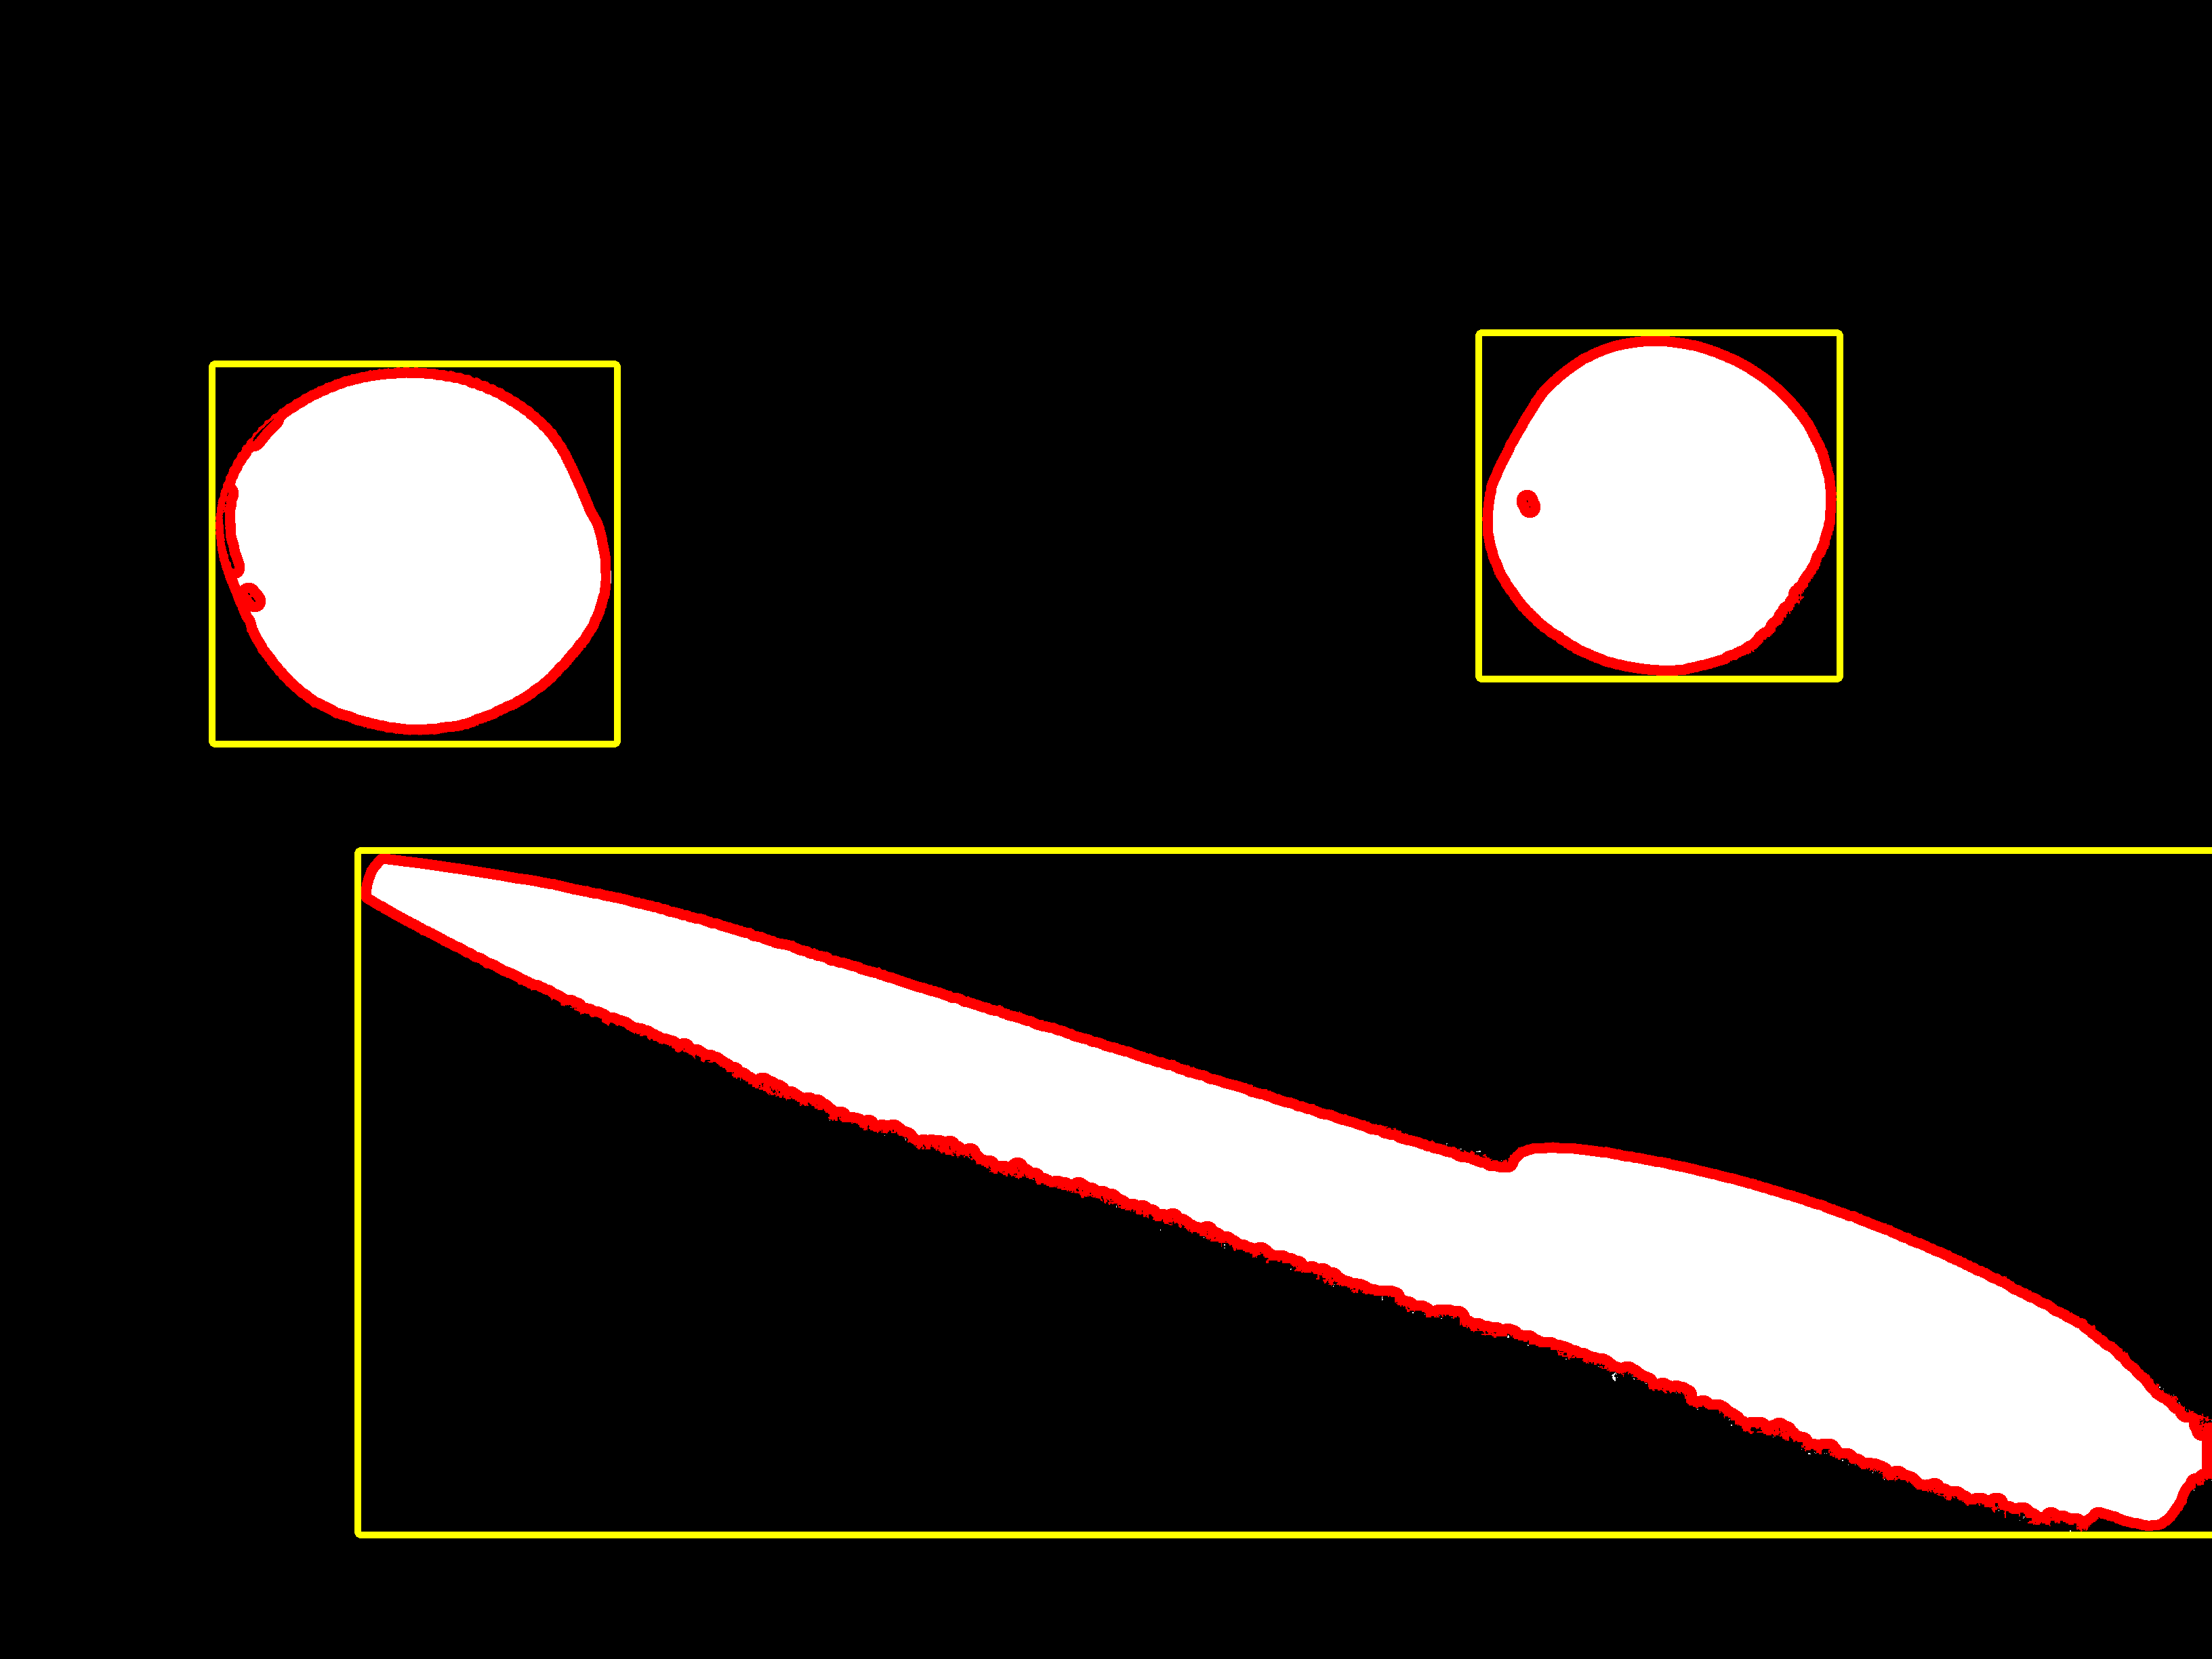
\includegraphics[width=\textwidth/2]{Bilder/Software/ColormodelsSegmentated}
\caption{Beispiel einer Segmentierung des binarisierten Sättigungskanals}
\label{fig:SegmentedColorModels}
\end{figure}

\section{Objektverfolgung}

Sobald ein Objekt durch die in Kapitel \ref{sec:Objekterkennung} dargestellten Algorithmen erkannt wurde, so muss sichergestellt werden, dass die Fokussierung auf dieses Objekt beibehalten werden kann. Ein zufälliges Umspringen auf zufällige andere erkannte Objekte wäre für den Prozess sehr hinderlich. In den folgenden Abschnitten sind Kriterien und Probleme beschrieben, an Hand derer ein erkanntes Objekt in folgenden Bildern erkannt werden kann.

\subsection{Ähnlichkeitskriterien}

Um den Fokus auf ein Objekt zu behalten lassen sich verschiedene Ähnlichkeitskriterien formulieren durch die das erkannte Objekt in der Menge der im nachfolgenden Bild erkannten Objekte wieder gefunden werden kann.

\subsubsection{Lokale Nähe}
Das trivialste Kriterium stellt die lokale Nähe da. Geht man von einem Stillstand der Kamera und der aufgenommenen Szene aus, so befinden sich sämtliche Objekte in nachfolgenden Aufnahmen an der selben Stelle. Fokussierte Objekte können also rein aus ihrer Position wiedergefunden werden. Geschieht Bewegung, so kann nicht mehr von einer exakten Übereinstimmung der Koordinaten ausgegangen werden. Stattdessen muss eine gewisse Toleranz gegeben werden. Als Maß kann hierbei angenommen werden, dass sich die Position des Zentrums eines Objektes in fortlaufenden Aufnahmen um nicht mehr als beispielsweise 10\% der Aufnahmegröße geändert hat.

\subsubsection{Größenkriterium}
Das Größenkriterium ähnelt zunächst dem Kriterium der lokalen Nähe, bezieht sich jedoch nicht auf den Mittelpunkt des Objekts, sondern auf die vom Objekt in der Aufnahme eingenommenen Fläche. Diese bleibt bei einer beliebigen Translation des Objektes in der Aufnahme konstant und eignet sich daher als Ähnlichkeitsmaß. Bewegt sich das Objekt jedoch auf die Kamera zu, oder von ihr weg, so verändert sich die eingenommene Fläche. Auch hier muss eine Toleranz gewählt werden. Dise kann entweder konstant gegeben sein (beispielsweise 10\%) oder abhängig von der aktuellen Geschwindigkeit des Roboters gewählt werden.


\subsubsection{Farbliche Ähnlichkeit}
Ein drittes Ähnlichkeitsmaß stellt die farbliche Ähnlichkeit dar. Diese ist Abhängig vom Farbraum in dem die Aufnahme getätigt oder konvertiert wurde. Wie in Abschnitt \ref{sec:Objekterkennung} beschrieben, wird die Aufnahme bei der Objekterkennung in das HSV-Format konvertiert. Daher kann das Ähnlichkeitsmaß sich auf den Farbkanal, den Sättigungskanal oder den Intensitätskanal beziehen. Durch außschließen des Intensitätskanals kann eine weitgehend helligkeitsunabhängige Bestimmung erreicht werden. Daher ist das Filtern nach Objekten ähnlicher Farbe und Sättigung durchaus sinnvoll. Auch hier lässt sich eine Toleranz formulieren, wie etwa 10\% Abweichung von der durchschnittlichen Farbe des zuvor ermittelten Objektes.


\subsection{Kurzzeitiges Verlieren eines Objektes}
\subsection{Verschwommene Bilder durch Bewegung des Roboters}

\section{Entfernungsschätzung}
Die Entfernungsschätzung ist für mehrere Teile der Roboterroutine wichtig. Zunächst muss der Roboter, der ein Objekt per Kamera erkannt hat anfahren und aufheben. Hierfür muss er wissen ob der aufzuhebende Gegenstand in Reichweite des Greifarms ist. Weiterhin benötigt der Roboter die Entfernungsschätzung bei der Navigation. Er muss Hindernisse, wie beispielsweise Wände eines Raumes, erkennen bevor er kollidiert und unter Umständen seine Fracht verliert.

\subsection{Stereokamerabasiert}
\label{subsec:StereoKameraDist}

Ein häufiger Ansatz für die Entfernungsschätzung stellt die Stereokamerabasierte Methode dar. Hierbei nimmt der Roboter seien Umgebung nicht mit nur einer Kamera, sondern mit mehreren, mindestens zwei, wahr. Durch einen bekannten Versatz zwischen den Aufnahmequellen der Bilder, lässt sich mittels Registrierung auch ein Versatz in den erzeugten Bildern ermitteln. Wie die beiden menschlichen Augen, erlaubt dies das Wahrnehmen der Umgebung in dritter Dimension. Abbildung \ref{fig:StereokameraEntfernung} zeigt exemplarisch eine solche Entfernugnsschätzung.

\begin{figure}[h]
\centering
\caption{Stereokamerabasierte Entfernungsschätzung}
\label{fig:StereokameraEntfernung}
\end{figure}

Der Stereokamerabasierte Ansatz ist von der Ausführung sehr elegant, da er sich an der Natur orientiert. Problematisch ist jedoch, dass zusätzliche Hardware benötigt wird. Eine weitere Kamera als bildgebendes Mittel birgt einen neuen Grad der Komplexität, da diese mit dem vorhandenen Smartphone synchronisiert werden muss. Zusätzlich müssen Rechenintensive Registrierungen vorgenommen werden, wodurch die Echtzeitfähigkeit des Systems beeinträchtigt werden könnte.

[HIER FEHLT NOCH EINE QUELLE]


\subsection{Monokamerabasiert}

Der Monokamerabasierte Ansatz stützt sich auf allen vorhandenen Informationen. Hierbei wird mittels der bekannten Position und Inklination der Kamera, sowie ihres Streuwinkels ein virtuelles Blickfeld erstellt. Dieses Blickfeld breitet sich von der Kamer aus pyramidenfärmig aus und trifft den als planar angenommenen Boden. Abbildung \ref{fig:MonokameraEntfernung} zeigt den Aufbau eines solchen Systems. 

\begin{figure}[h]
\centering
\caption{Monokamerabasierte Entfernungsschätzung}
\label{fig:MonokameraEntfernung}
\end{figure}

Anhand der Position des detektierten Objektes im Kamerabild lässt sich daraufhin eine ungefähre Entfernungsschätzung liefern. Problematisch ist hierbei die Ungenauigkeit des Systems. Sowohl Fehler bei der Aufnahme, als auch Probleme durch eine maximale Größenbeschränkung des detektierten Objektes können in der Praxis zu Fehleinschätzungen und damit fehlerhafter Benutzung des Greifarms führen.

[HIER FEHLT NOCH EINE QUELLE]

\subsection{Ultraschallbasiert}

Die Ultraschallbasierte Entfernungsschätzung kann auch über Große Distanzen von bis zu zwei Metern zentimetergenaue Entfernungen messen. Die Messung wird durch einen Echo-Mechanismus mit, für den Menschen unhörbaren, Schallwellen im Ultraschallbereich durchgeführt. [HIER FEHLT NOCH EINE QUELLE] Zunächst wird jedoch, ähnlich dem in \ref{subsec:StereoKameraDist} beschriebenen Verfahren, zusätzliche Hardware in Form eines Ultraschallsensors benötigt. Ein solcher kann jedoch direkt von LEGO\texttrademark erworben und problemlos am Roboter angebracht werden. 

Das Ultraschallbasierte Verfahren kann durch eine kleine Änderung des Roboters realisiert werden und liefert sehr genaue Ergebnisse. Die Koppelung mit dem Smartphone ist bereits gegeben und genügt daher Echtzeitanforderungen. 
\section{Raumerkennung}
\subsection{Kameragestützt}
\subsection{Streckenbasiert}
Über gefahrene Strecke
\subsection{Kombination unterschiedlicher Sensordaten}


\section{Zielzonenerkennung}


\section{Hauptschleife}

Arbeitszustände
\begin{enumerate}
\item{Objekt suchen}
\item{Objekt ansteuern}
\item{Objekt aufnehmen}
\item{Objekt kategorisieren}
\item{Zielbereich suchen}
\item{Zielbereich ansteuern}
\item{Objekt ablegen}
\end{enumerate}

[INSERT ZUSTANDSÜBERGANGSDIAGRAMM]
Petrinetz?

